%%
%% Author: Dario Chinelli
%% begin 2019-12-04
%% last mod 2022-02-02
%%

% Preamble
\documentclass[class=article, crop=false]{standalone}

% Packages
\usepackage[subpreambles=true]{standalone}
\usepackage{import}
\usepackage{graphicx}
\usepackage{amsmath}

% Document
\begin{document}

% Simulations documentation here


\FloatBarrier
\paragraph{Probability distribution}
The tool used in this work is a \emph{move probability} tensor.
For each position, and eventually also time, it returns a number between $0$ and $1$ for each element.
The sum over every directions must be $1$, because of the normalization.
This tensor is multidimensional, as described in the previous paragraphs, and its dimension depends on the model.
With this tool is possible to plot the map with the corresponding probability for each of the nine directions.
It is possible to see along the trajectories where is the more probable direction to take and which is the less.
To describe this lets take into account just a few real trajectories, with a common path and and opposite directions.
To do so, here are considered five pedestrians in (Figure \ref{fig:5pids_trjl}), with two representations:
one is plotting the actual lines in the field (Figure \ref{fig:5pids_trjlines}) and the other is a heat-map that describes where pedestrians passed through (Figure \ref{fig:5pids_trjlhist}).
\begin{figure}[h]
    \centering
    \subfloat[Trajectories lines of five "real" pedestrians.]{
        \label{fig:5pids_trjlines}
        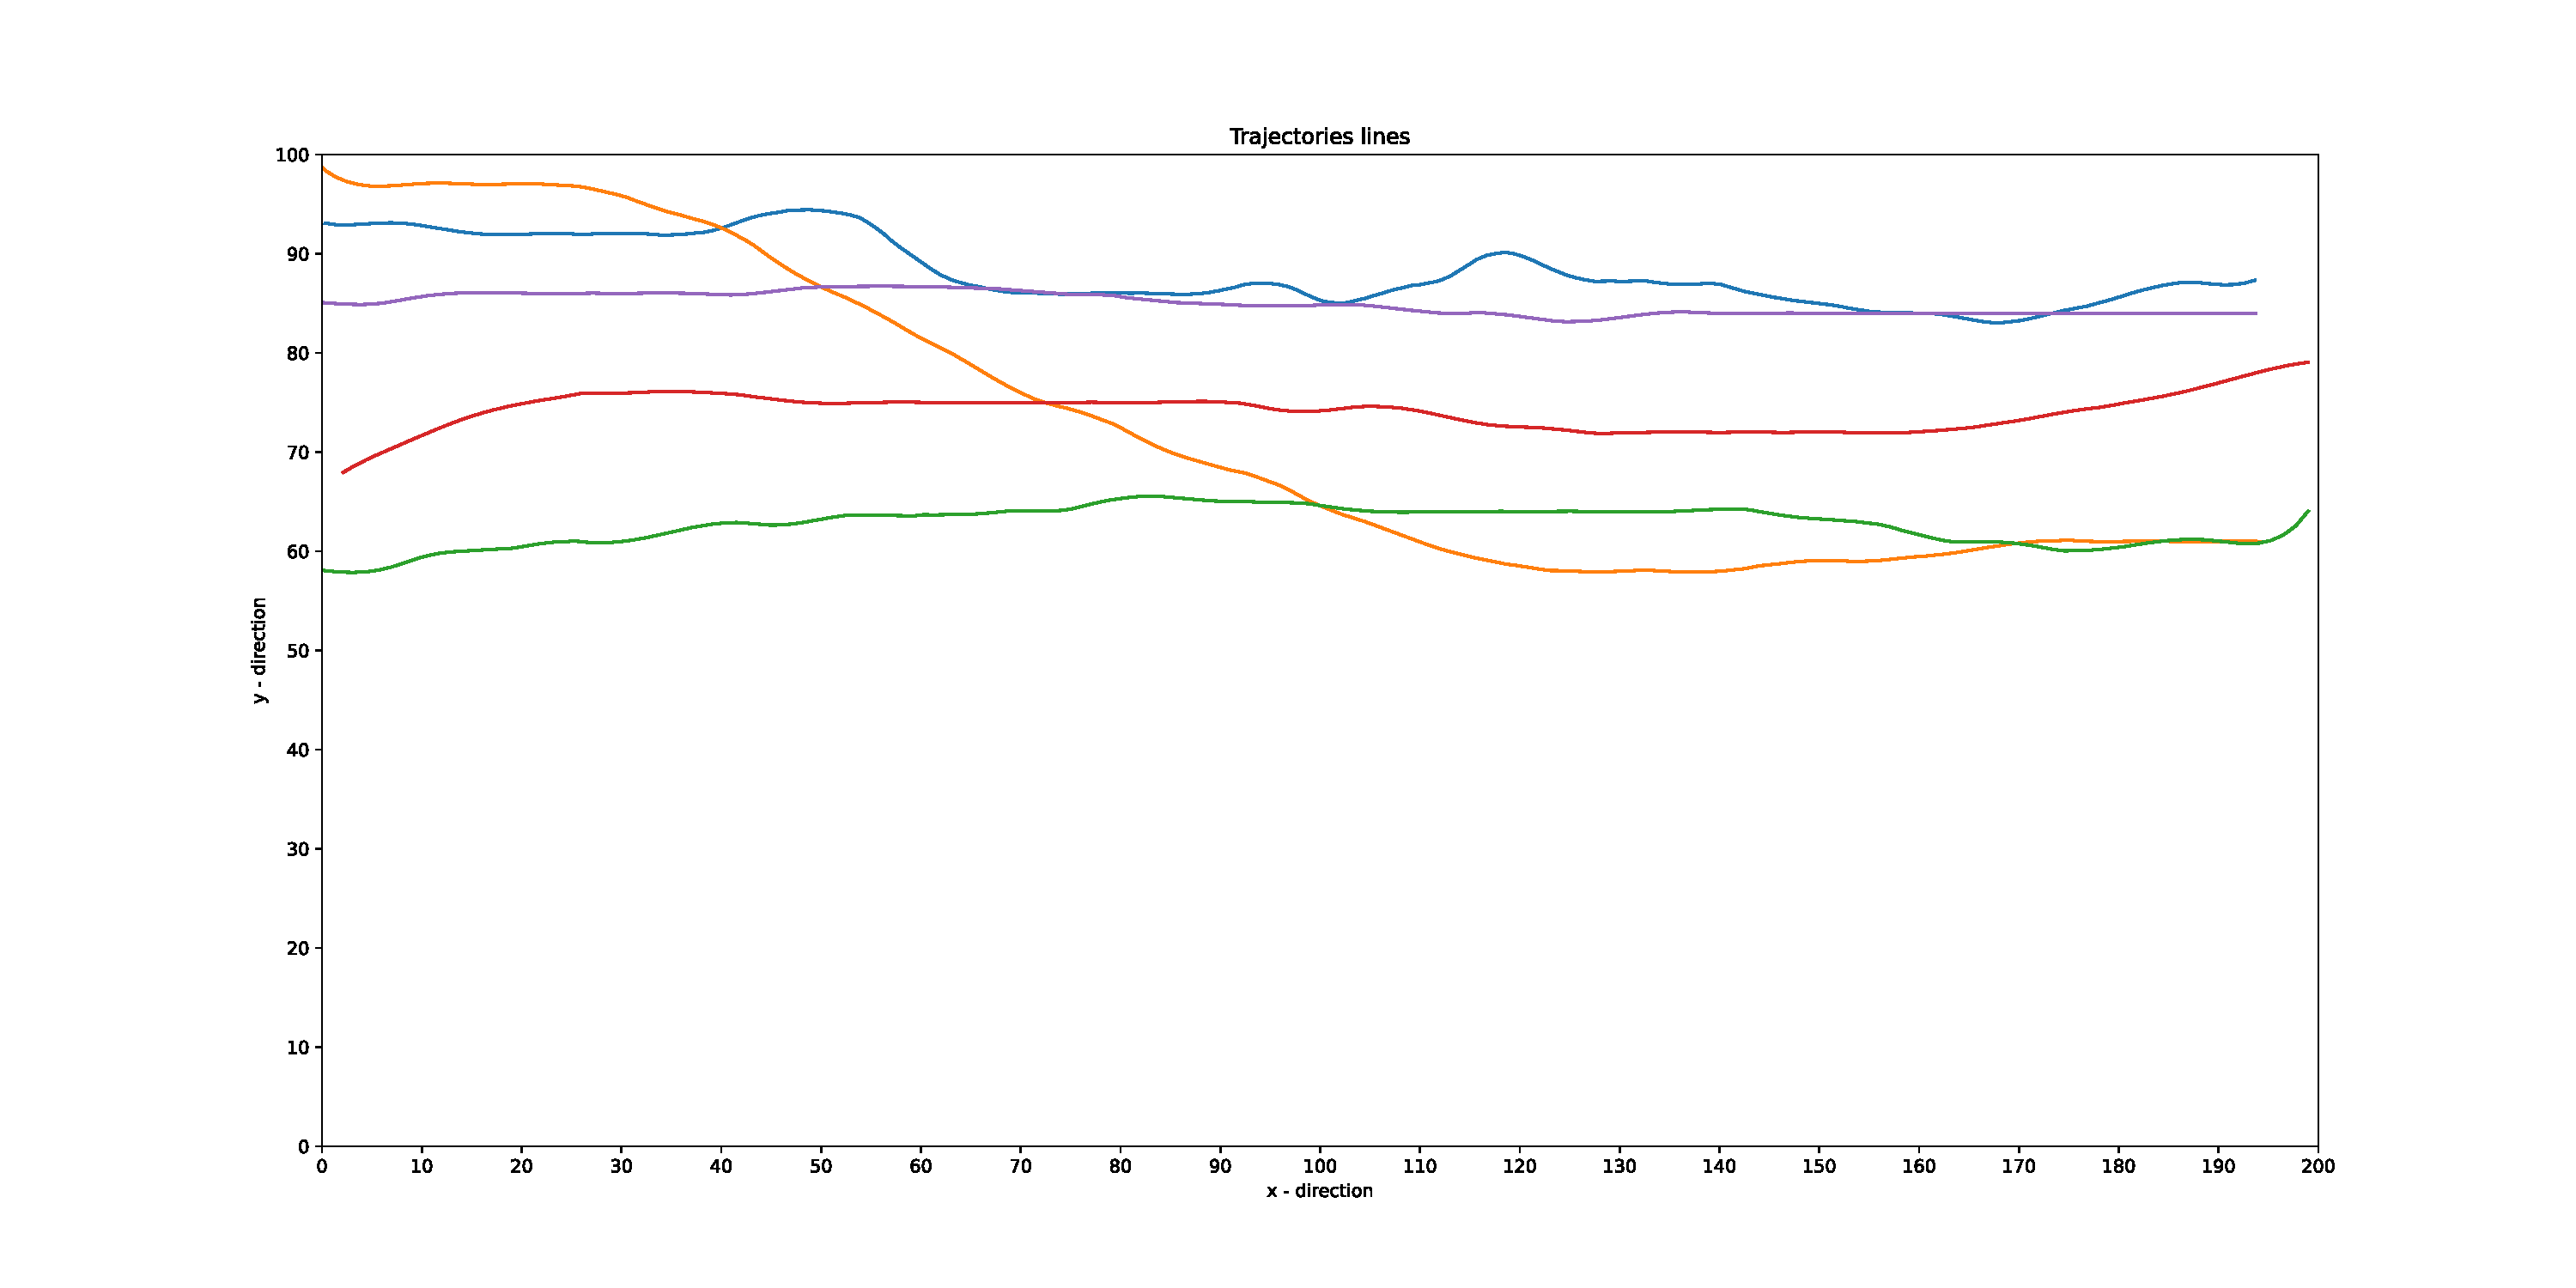
\includegraphics[ width=0.45\textwidth]{fig/5pids/figure_trainf10_few_trajectories_Dx200_Dy100_TRJLINES}
    }\quad
    \subfloat[Trajectories heatmap of five "real" pedestrians.]{
        \label{fig:5pids_trjlhist}
        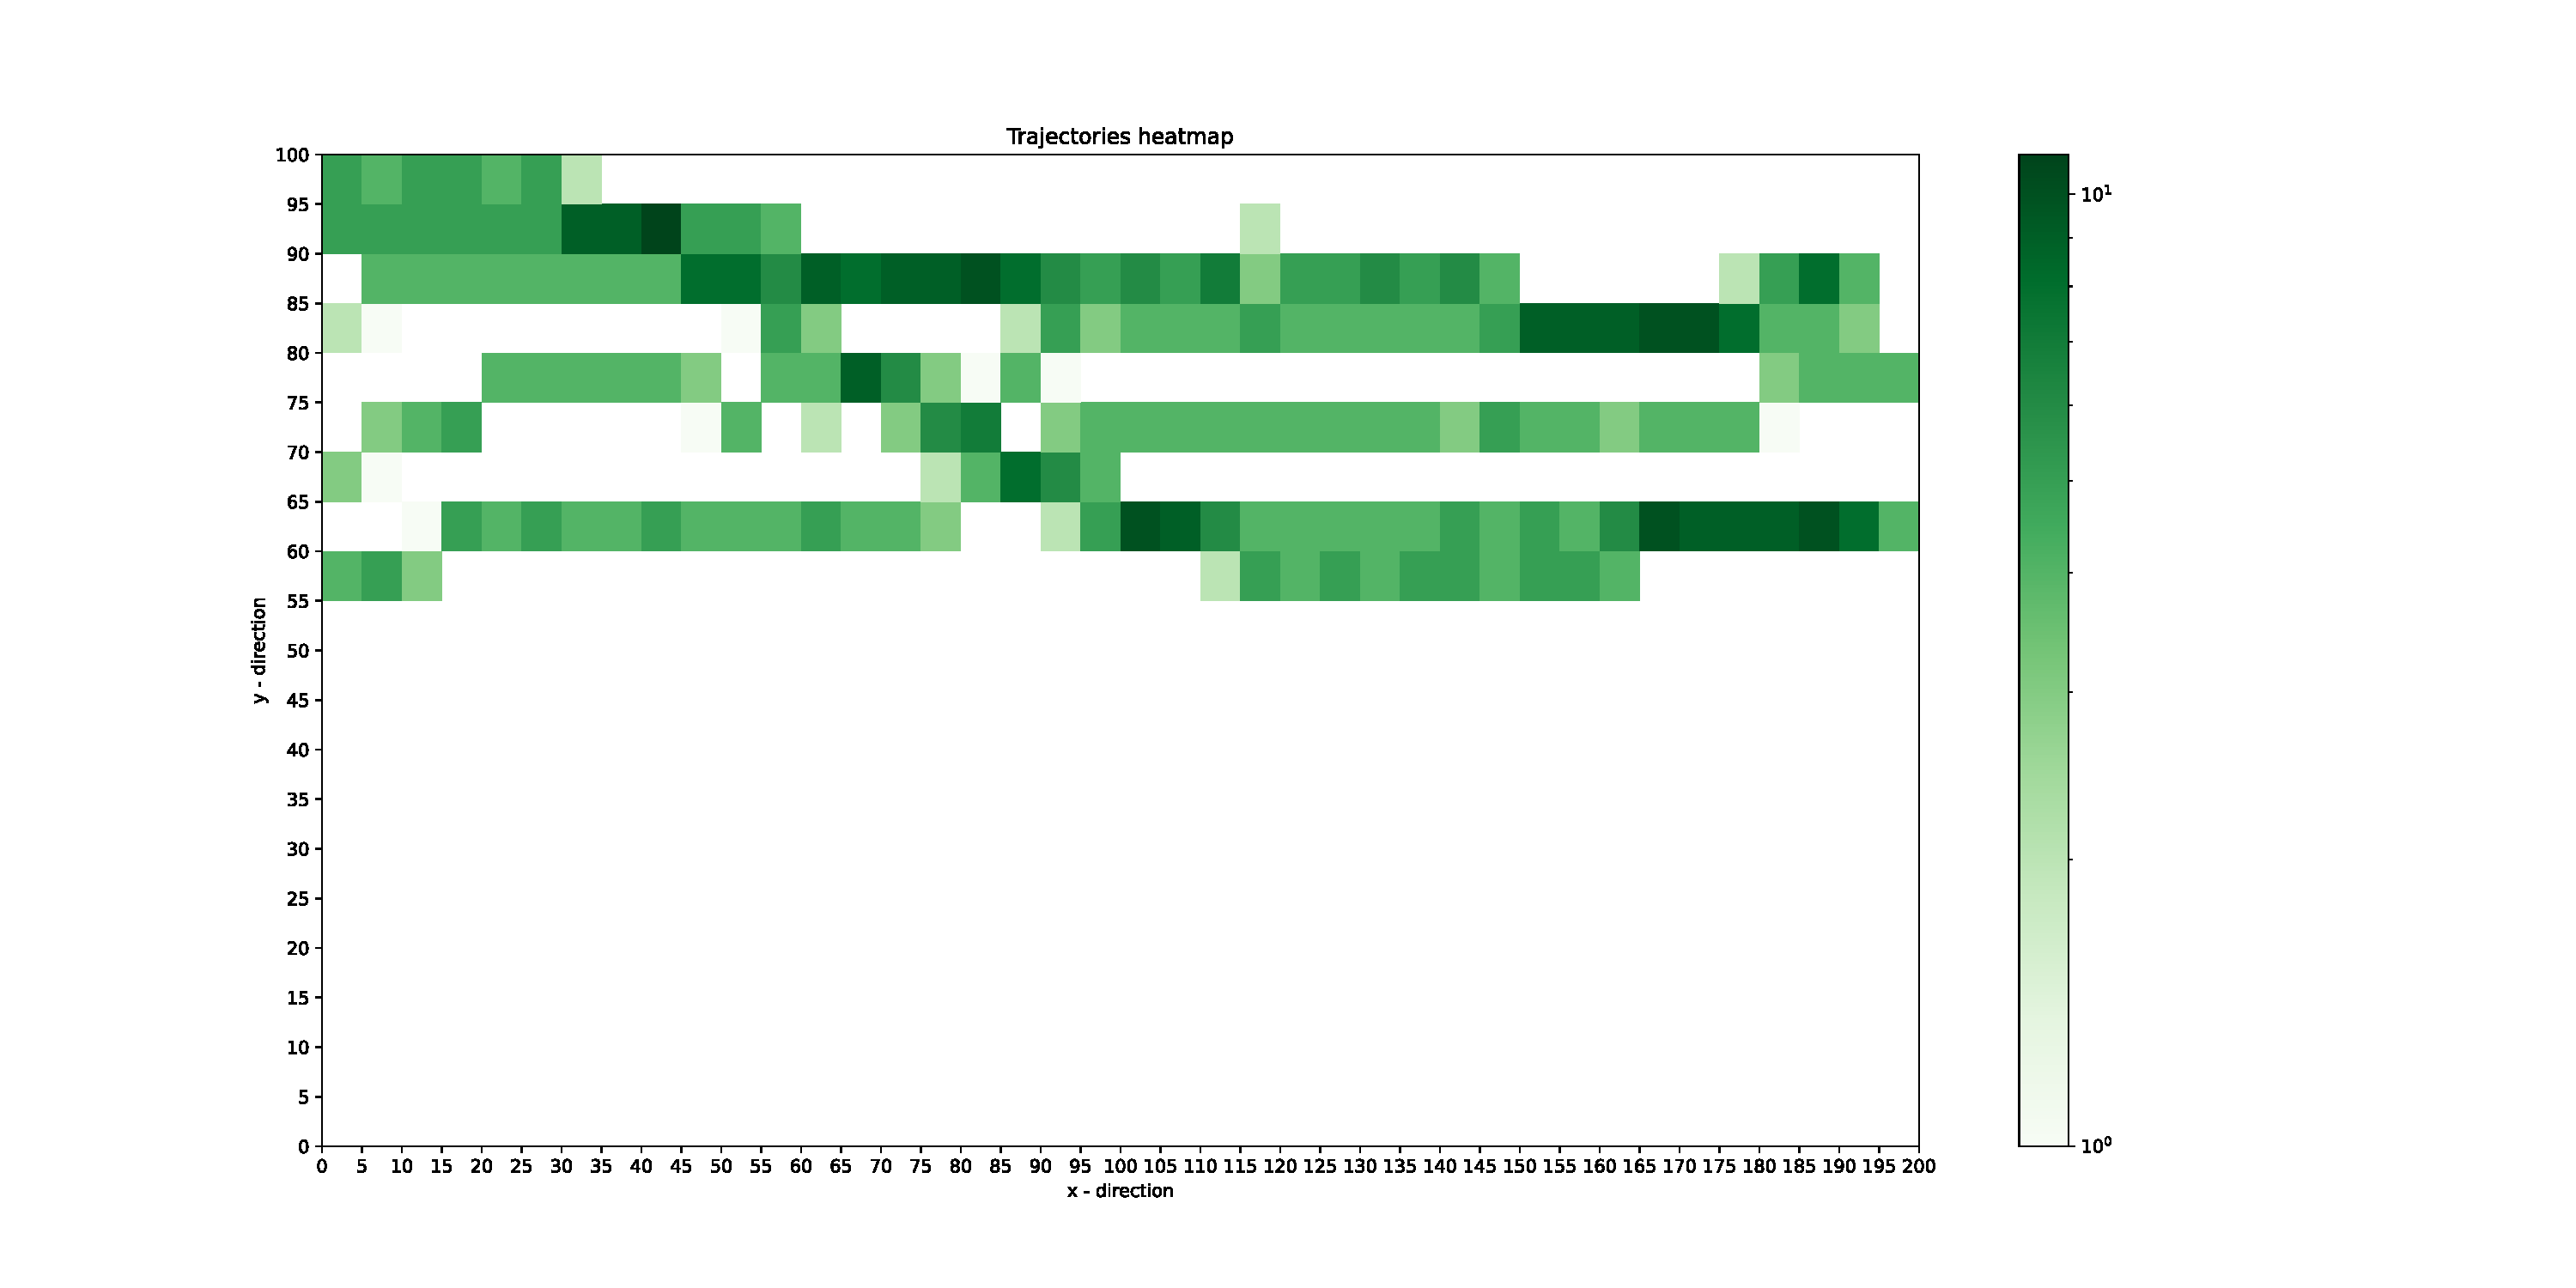
\includegraphics[ width=0.4\textwidth]{fig/5pids/figure_trainf10_few_trajectories_Dx200_Dy100_TRJHIST}
    }
    \captionsetup{width=.8\linewidth}
    \caption{Representation of five real trajectories from dataset.}
    \label{fig:5pids_trjl}
\end{figure}
\paragraph{Velocities plot}
A significant plot to understand those paths is the one that compare the velocity along the two axes $x$ and $y$.
In this example it describes how some trajectories are walking left and others are going right, see the (Figure \ref{fig:5pids_velhist}).
This plot is made as heat-map, that means each cell gives the intensity of that unique combination of velocities.
\begin{figure}[h]
\centering
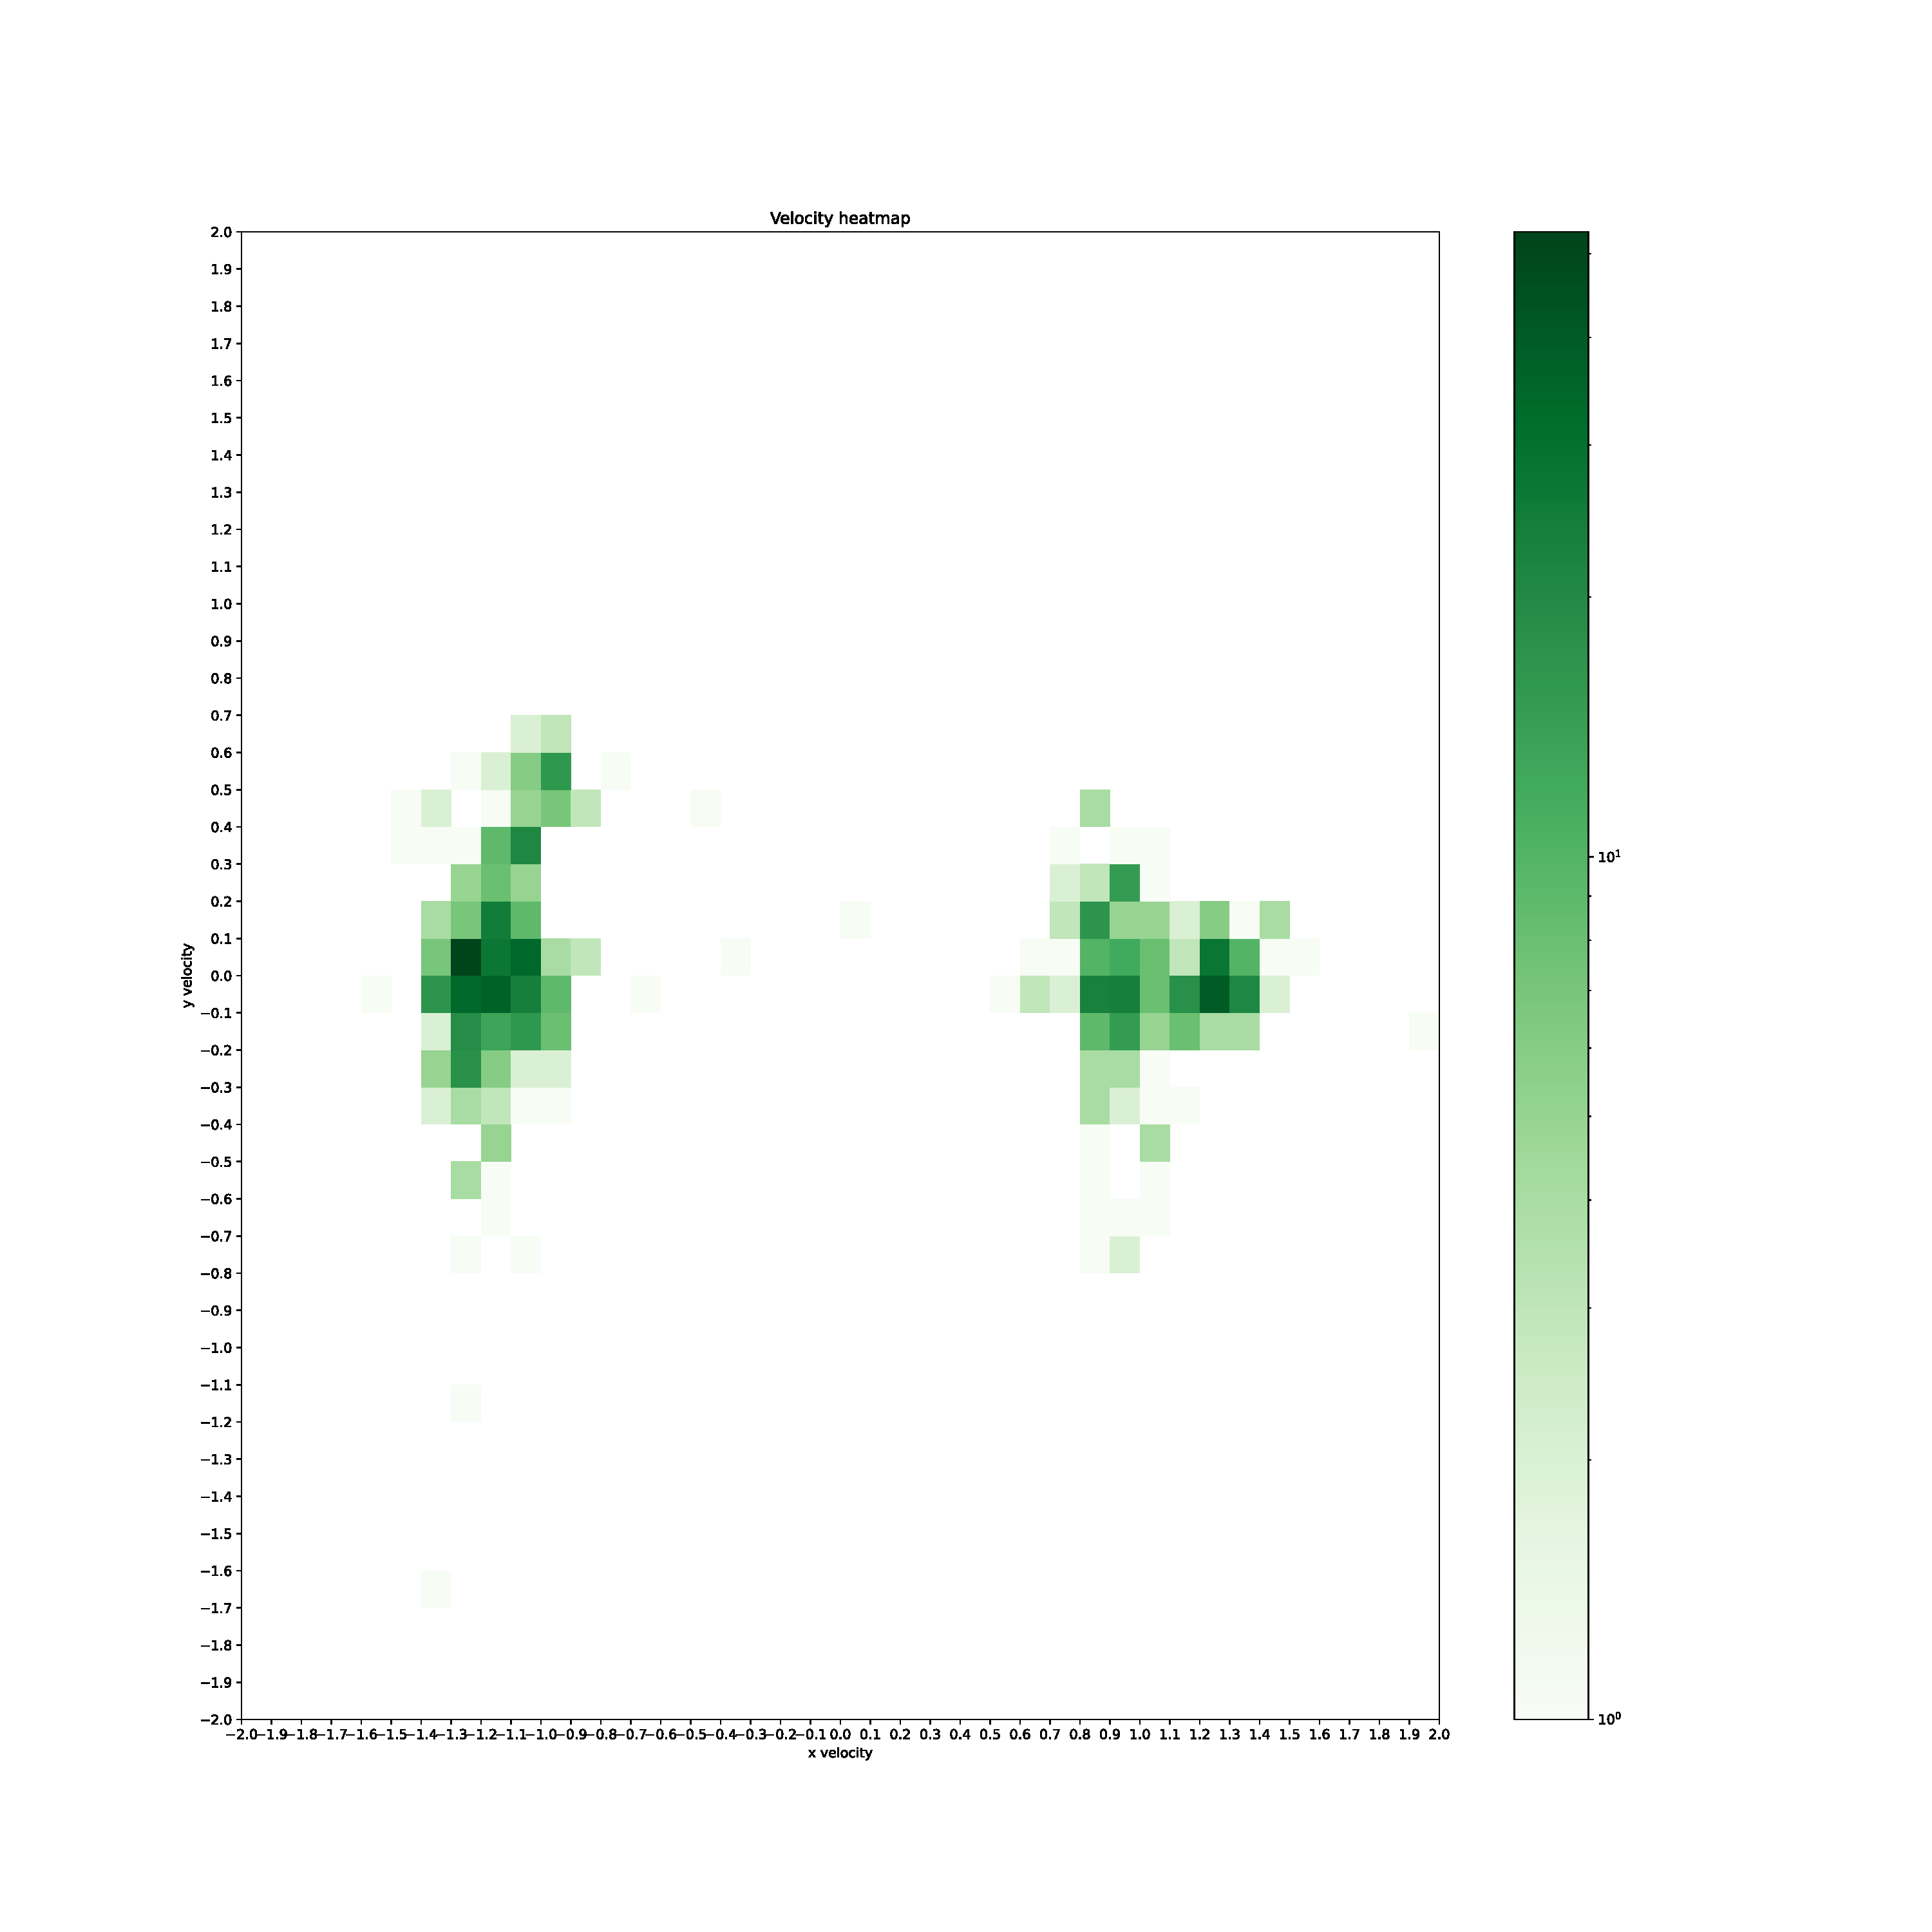
\includegraphics[scale=0.2]{fig/5pids/figure_trainf10_few_trajectories_Dx200_Dy100_VELHIST}
\captionsetup{width=.5\linewidth}
\caption{Comparison between velocity along the two directions $v_x$ and $v_y$.}
\label{fig:5pids_velhist}
\end{figure}
\paragraph{D2Q9 representation}
Another significant plot is the $3\times3$ matrix of figures that follows in (Figure \ref{fig:5pids_D2Q9}), it is composed by nine images.
All those images are referred to the same field, with the same dimensions.
In each of those is plotted the move probability along just one direction.
The positions of those images is oriented as the $D2Q9$ map, showed in (Figure \ref{fig:D2Q9_k}).
So that the center figure represents the probability to stand still, meanwhile the right-center figure is the probability to move right and so on.
\begin{figure}[h]
\centering
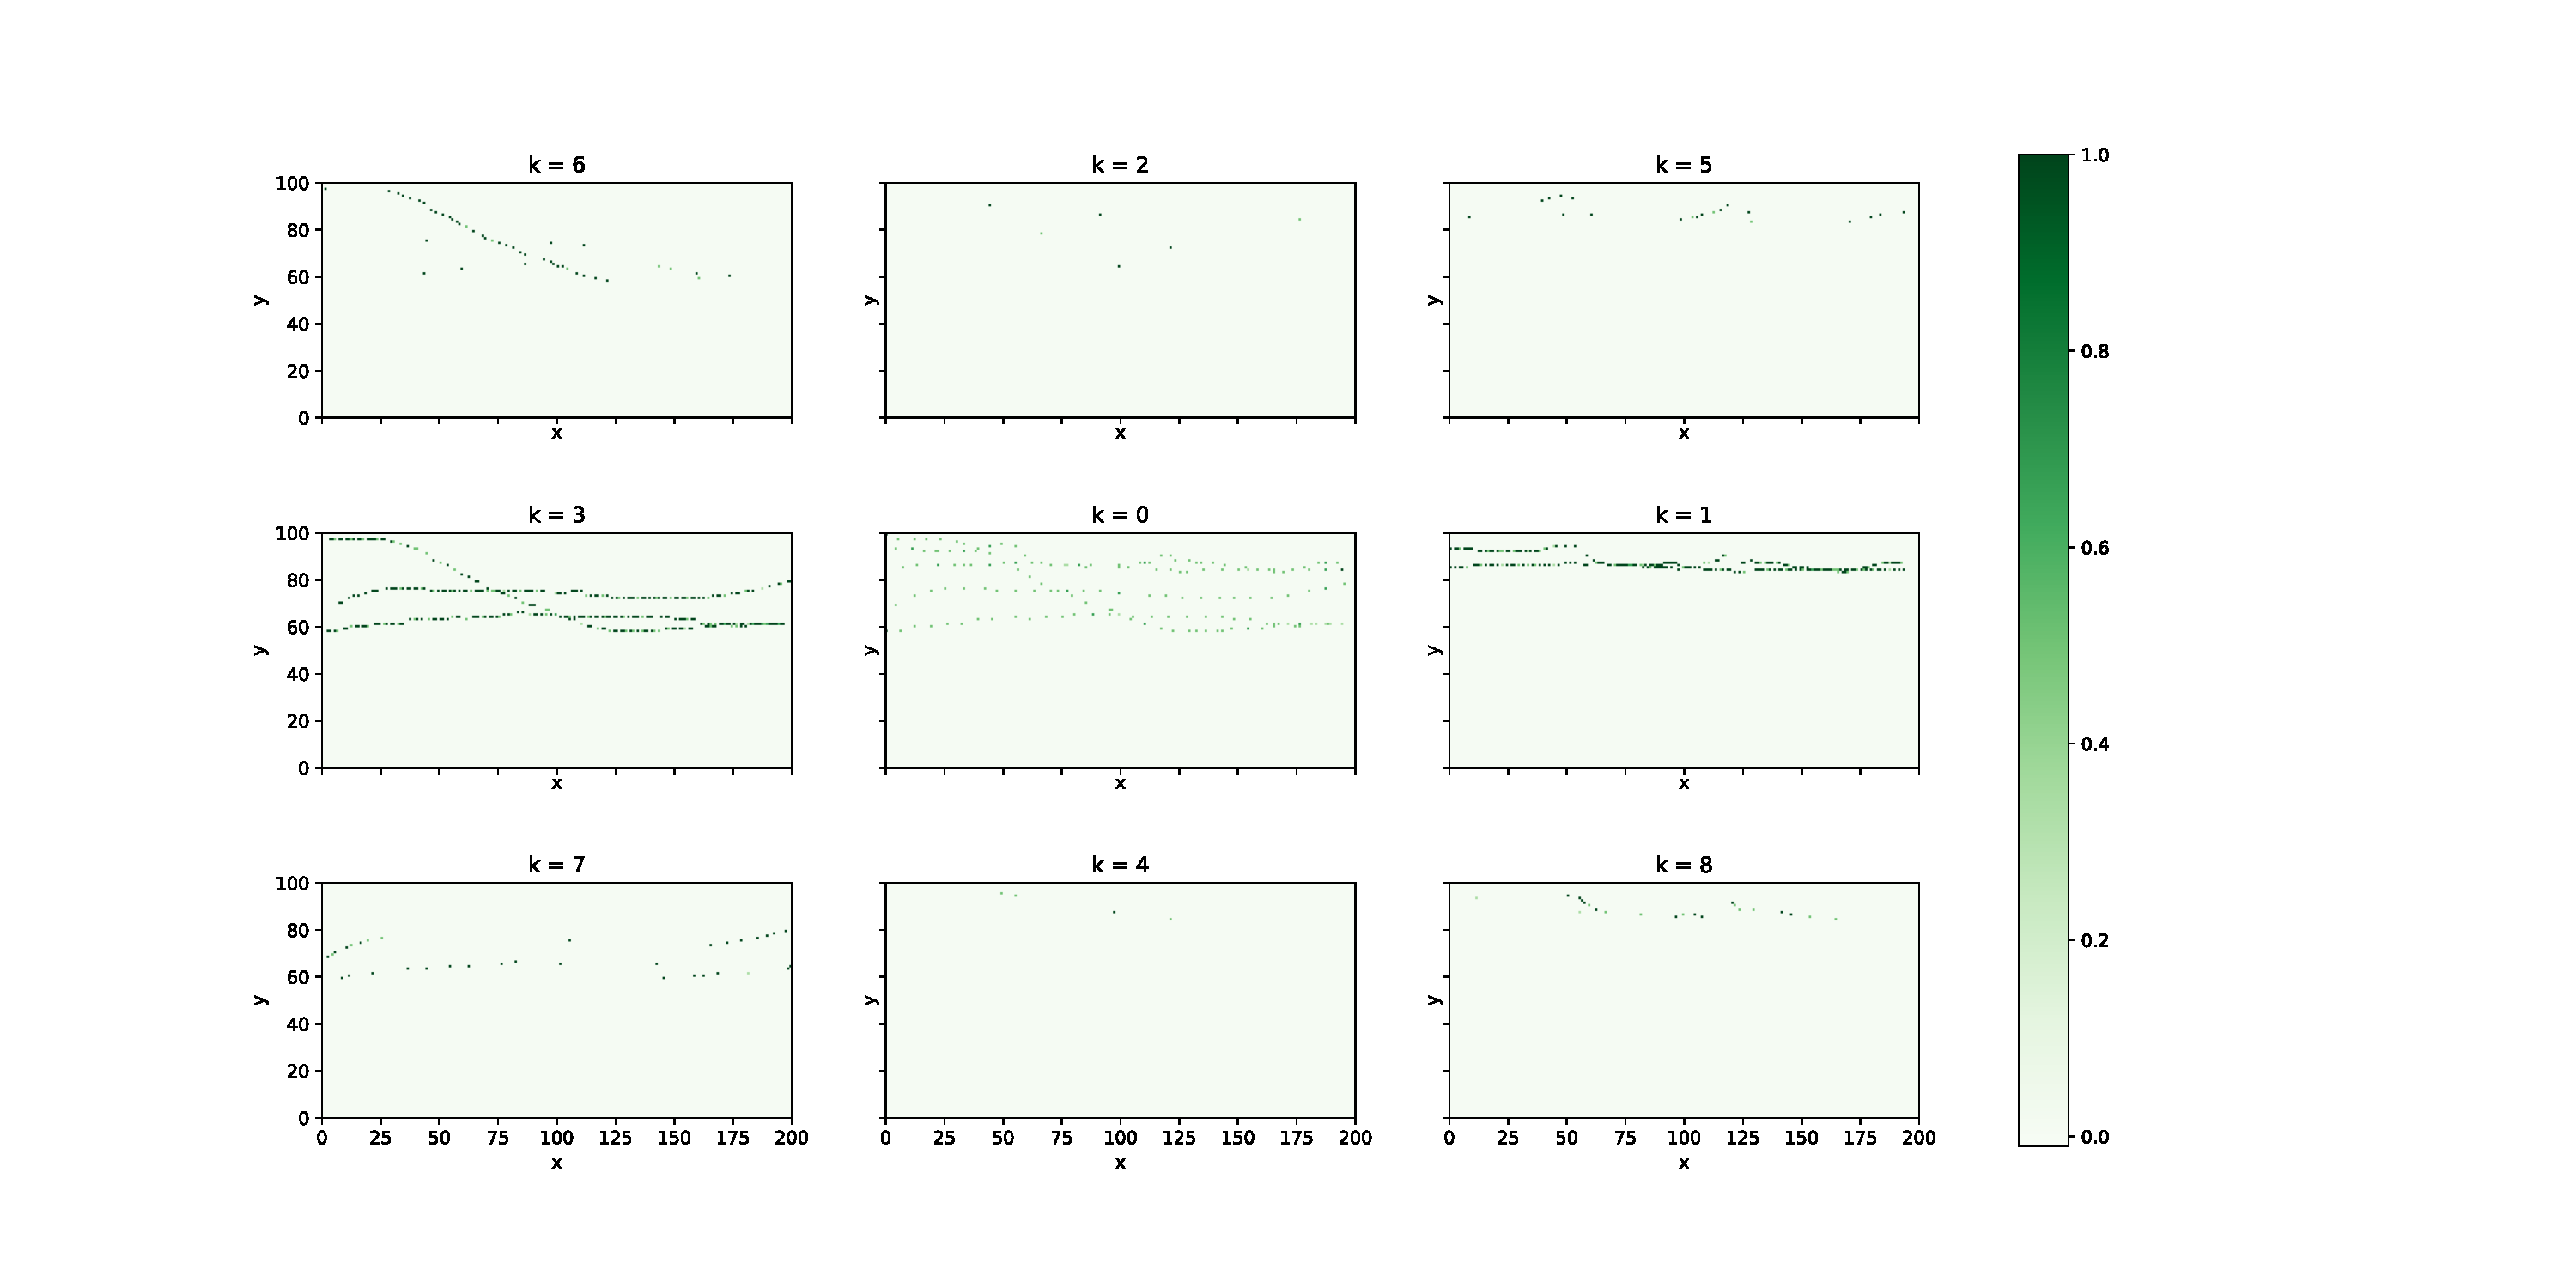
\includegraphics[scale=0.35]{fig/5pids/figure_trainf10_few_trajectories_Dx200_Dy100_D2Q9}
\captionsetup{width=.6\linewidth}
\caption{Representation of the D2Q9 model. Every plot shows the move probability for each associated direction.}
\label{fig:5pids_D2Q9}
\end{figure}




\FloatBarrier
\subsection{Trajectories simulation}
The aim of a good simulation is to be capable of recreate a realistic path.
In other words, the aim is to make a good prediction on the path chosen by a pedestrian.
To do so, it is necessary to \emph{understand} the trajectories, to \emph{learn} the motion from real life experiment, before trying to simulate it.

\paragraph{Start positions}
The first step is always the hardest to make, others follows.
The simulation has a start on a cell that is considered part of an group of cells with certain characteristics.
To define this group is necessary to analyze where a real life trajectory start.
Lets consider a raw trajectory, a discrete path made from consecutive points.
At every time is associated a position on the $x$ ax and on the $y$ ax.
So that a trajectory is described as a group of points in three dimensions, one in time and to in space.
With this definition is easy to define a starting position, asking where is the position when the time is minimum.
The group of the possible \emph{start positions} is created going through all the trajectories and select the points that correspond to the minimum time for each of those.

Once the group of start position is created, it is possible to assign to a synthetic pedestrian its initial position.
In this work the assignation is made by a random sort from the group of named before.
It is possible to select a region of interest in the field.
Combining an arbitrary portion of space and the group of start position and making a new sub-group.
Than the random choose is made from that secondary sub-group.

\paragraph{Step}
The step from the initial position to the second is essentially made with the same procedure as all further steps.
The algorithm take as input the position, in space and time if necessary.
The tensor $A$ is used to get the probability for each of the nine directions.
So that the initial position, chosen from the group of the start positions, is associated to the time $t=0$.
When this input is given to the algorithm it read the array of the possible transitions from the actual cell to the next.
Then it run a Monte Carlo trough that array and returns the corresponding direction randomly chosen with different probabilities.

Here some examples to explain the algorithm.
The (Figure \ref{fig:D2Q9_FirstEx}) represents a scenario where in a certain position it is associated a distribution of probability that make certain the evolution of the system.
In the figure is described that is not possible to move anywhere except to the Right direction.
For the second example in (Figure \ref{fig:D2Q9_SecondEx}) is given a different probability distribution.
If in a certain position $(x_0, y_0)$ is associated this type of distribution the randomization will be between going Right or going Down with the same probability.
For the third example in (Figure \ref{fig:D2Q9_thirdEx}) lets assume every entry non-zero.
In this case some of the future positions will have a really low probability to happen and others very high.
So that simulating a great number of trajectories will lead to get some of them "choosing" also the less probable directions.
For sure the most probable choice is to go Right, the second is to go Down and the third in order of probability is to go Right-Down.
All the other directions follows as less probable, but with a non-zero probability.




\begin{figure}[ht]
\begin{minipage}[c]{0.33\linewidth}
\centering
\resizebox{0.7\textwidth}{!}{%
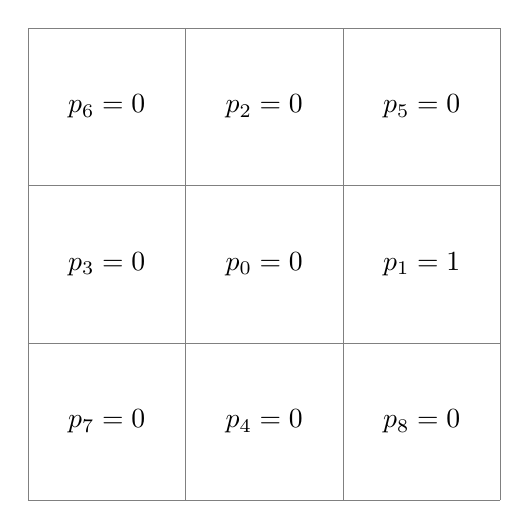
\begin{tikzpicture}
% Lines
\draw[step=2cm, gray, very thin] (0,0) grid (6,6);
% Nodes
\draw (3,3) node[black] {$p_0 = 0$};
\draw (5,3) node[black] {$p_1 = 1$};
\draw (3,5) node[black] {$p_2 = 0$};
\draw (1,3) node[black] {$p_3 = 0$};
\draw (3,1) node[black] {$p_4 = 0$};
\draw (5,5) node[black] {$p_5 = 0$};
\draw (1,5) node[black] {$p_6 = 0$};
\draw (1,1) node[black] {$p_7 = 0$};
\draw (5,1) node[black] {$p_8 = 0$};
\end{tikzpicture}
}%
\captionsetup{width=.8\linewidth}
\caption{First example of probability distribution for a certain position. Always right.}
\label{fig:D2Q9_FirstEx}
\end{minipage}
\begin{minipage}[c]{0.33\linewidth}
\centering
\resizebox{0.7\textwidth}{!}{%
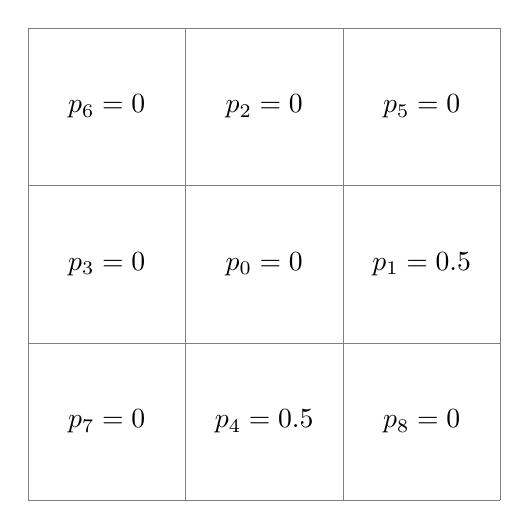
\begin{tikzpicture}
% Lines
\draw[step=2cm, gray, very thin] (0,0) grid (6,6);
% Nodes
\draw (3,3) node[black] {$p_0 = 0$};
\draw (5,3) node[black] {$p_1 = 0.5$};
\draw (3,5) node[black] {$p_2 = 0$};
\draw (1,3) node[black] {$p_3 = 0$};
\draw (3,1) node[black] {$p_4 = 0.5$};
\draw (5,5) node[black] {$p_5 = 0$};
\draw (1,5) node[black] {$p_6 = 0$};
\draw (1,1) node[black] {$p_7 = 0$};
\draw (5,1) node[black] {$p_8 = 0$};
\end{tikzpicture}
}%
\captionsetup{width=.8\linewidth}
\caption{Second example of probability distribution for a certain position. Always right or down.}
\label{fig:D2Q9_SecondEx}
\end{minipage}
\begin{minipage}[c]{0.33\linewidth}
\centering
\resizebox{0.7\textwidth}{!}{%
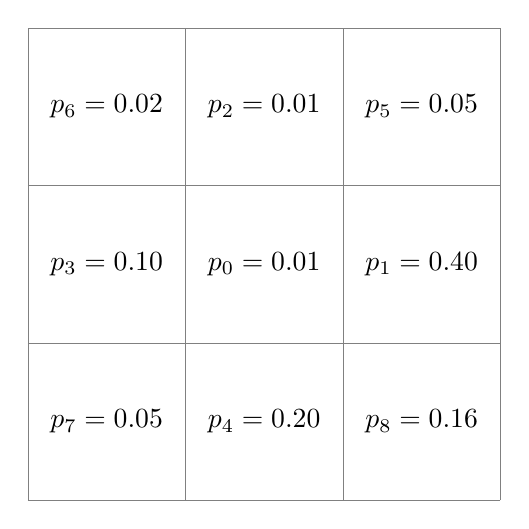
\begin{tikzpicture}
% Lines
\draw[step=2cm, gray, very thin] (0,0) grid (6,6);
% Nodes
\draw (3,3) node[black] {$p_0 = 0.01$};
\draw (5,3) node[black] {$p_1 = 0.40$};
\draw (3,5) node[black] {$p_2 = 0.01$};
\draw (1,3) node[black] {$p_3 = 0.10$};
\draw (3,1) node[black] {$p_4 = 0.20$};
\draw (5,5) node[black] {$p_5 = 0.05$};
\draw (1,5) node[black] {$p_6 = 0.02$};
\draw (1,1) node[black] {$p_7 = 0.05$};
\draw (5,1) node[black] {$p_8 = 0.16$};
\end{tikzpicture}
}%
\captionsetup{width=.8\linewidth}
\caption{Third example of probability distribution for a certain position. None zero probability.}
\label{fig:D2Q9_thirdEx}
\end{minipage}
\end{figure}








\FloatBarrier
\subsection{Distribution simulation}











\end{document}
